%!TEX TS-program = xelatex
%!TEX encoding = UTF-8 Unicode

\documentclass[12pt]{extarticle}
% extarticle is like article but can handle 8pt, 9pt, 10pt, 11pt, 12pt, 14pt, 17pt, and 20pt text

\def \ititle {Origins of Mind}
 
\def \isubtitle {Lecture 08}
 
\def \iauthor {Stephen A. Butterfill}
\def \iemail{s.butterfill@warwick.ac.uk}
\date{}

%for strikethrough
\usepackage[normalem]{ulem}

\input{$HOME/Documents/submissions/preamble_steve_handout}

%\bibpunct{}{}{,}{s}{}{,}  %use superscript TICS style bib
%remove hanging indent for TICS style bib
%TODO doesnt work
\setlength{\bibhang}{0em}
%\setlength{\bibsep}{0.5em}


%itemize bullet should be dash
\renewcommand{\labelitemi}{$-$}

\begin{document}

%\raggedcolumns

\begin{multicols*}{3}

\setlength\footnotesep{1em}


\bibliographystyle{newapa} %apalike

%\maketitle
%\tableofcontents




%--------------- 
%--- start paste

\def \ititle {Logic I}
 
\def \isubtitle {Lecture 01}
 
\begin{center}
 
{\Large
 
\textbf{\ititle}: \isubtitle
 
}
 
 
 
\iemail %
 
\end{center}
 
Readings refer to sections of the course textbook, \emph{Language, Proof and Logic}.
 
 
 
\section{The Pigs of Logic}
 
\emph{Reading:} §1.1, §1.2, §2.1
 
\textbf{Argument 1:} \begin{quote} Either it went up the left fork or it went up the right fork.

It didn’t go up the left fork.

therefore:

It went up the right fork. \end{quote}

\textbf{Argument 2:} \begin{quote} Either it went up the left fork or it went up the right fork.

The left fork is unsuitable for pigs.

therefore:

It went up the right fork. \end{quote}

 
\begin{minipage}{\columnwidth}
 
\textbf{awFOL version of Argument 1:}
 
\begin{center}
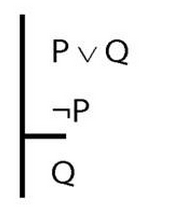
\includegraphics[scale=0.3]{img/argument1_fol.png}
\end{center}
\end{minipage}
 
 
 
\section{Why Logic?}
 
‘If a card has a vowel on one side, then it has an even number on the other side.’
(Waison \& Johnson-Laird 1972)
 
\begin{center}

\includegraphics[scale=0.3]{img/waison_fig.png}
\end{center}
‘Logic pervades the world: the limits of the world are also its limits.’
(Wittgenstein, Tractatus 5.61)
 
 
\section{Logic-Ex}
 
There are logic exercises associated with each lecture. After each lecture (or before, if you prefer), you should complete the associated exercises.
 
You can find links to the exercises for each lecture at: \url{http://logic-1.butterfill.com}
 
To complete the exercises you need to register at \url{http://logic-ex.butterfill.com} (If you don’t want to do this, you can complete the alternative textbook exercises on paper. These are also specified for each lecture at \url{http://logic-1.butterfill.com}).
 
Seminars will discuss exercises associated with the previous week’s lectures. As your seminar tutor will track your progress and mark your exercises, you should be sure to \textbf{complete the exercises by 2pm on the day before your seminar}.
 
 
 
 
\section{Quick Intro to awFOL}
 
\emph{Reading:} §1.1, §1.2, §1.3
 
 
\begin{center}
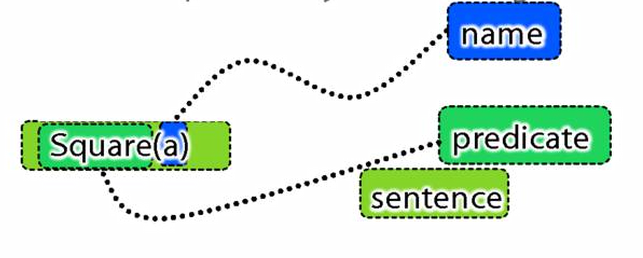
\includegraphics[scale=0.3]{img/name_predicate_sentence.png}
\end{center}
A formal langauge enables us to avoid ambiguity, e.g.:
 
\begin{quote}
 
This is a hospital where doctors are trained.
 
\end{quote}
 
A formal langauge also enables us to some avoid appearance--reality problems:
 
\begin{quote}
 
Many more people have been to Paris than I have.
 
\end{quote}
 
 
 
 
 
\section{Logically Valid Arguments}
 
\emph{Reading:} §2.1
 
An argument is \emph{logically valid} just if there’s no possible situation in which the premises are true and the conclusion false
 
A \emph{connective} joins one or more sentences to make a new sentence. E.g. ‘because’, ‘¬’. The sentences joined by a connective are called \emph{constituent sentences}.
 
E.g. in ‘P $\lor{}$ Q’,
 
\begin{quote}
 
$\lor{}$ is the connective
 
P, Q are the constituent sentences
 
\end{quote}
 
\begin{center}
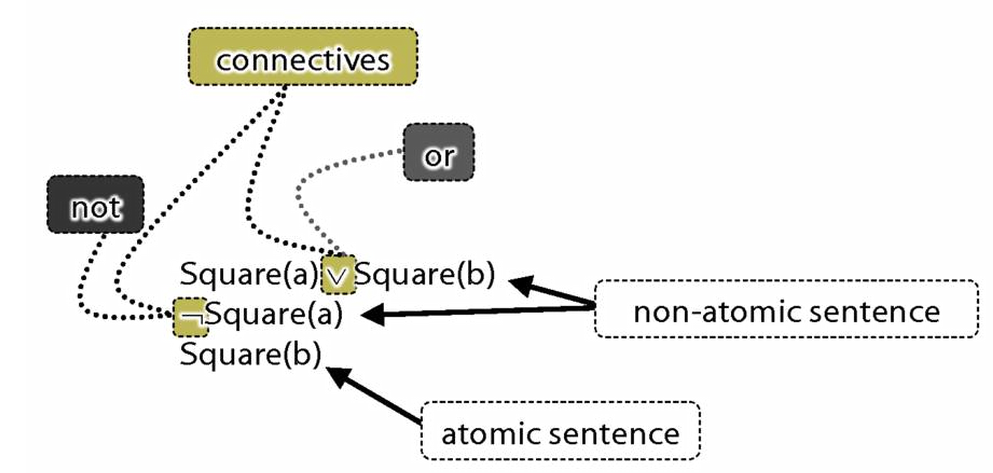
\includegraphics[scale=0.3]{img/terminology_more.png}
\end{center}
 
 
\section{Counterexamples}
 
\emph{Reading:} §2.5
 
A \emph{counterexample} to an argument is a possible situation in which its premises are T and its conclusion F.
 
There are no counterexamples to a logically valid argument.
 
If an argument is not valid, then there is a counterexample to it.
 
To show that an argument is not logically valid, we specify a counterexample to it.
 
%--- end paste
%--------------- 
 

\end{multicols*}

\end{document}